\section{Applying LIME}
\nblink{nhs-chest-xray/analyze/lime.ipynb}

Implementing LIME on the NIH Chest X-ray dataset with the DenseNet model was straightforward. The refence implementation is published on PyPI (Python Packaging Index) and can be installed with the pip Python package manager. Examples how 



, because the reference implementation of RISE on GitHub \cite{risegithub} already
containes a working implementation for PyTorch. The implementation was not published on the Python Packaging Index, so the code had to be downloaded and added into our GitHub repository.


\subsection{Results}
\begin{figure}[H]
\centering
\caption{Scan 0 LIME output}
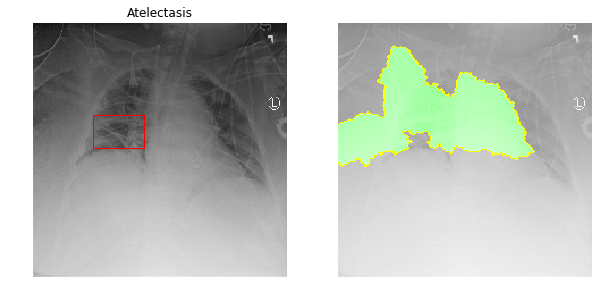
\includegraphics[width=12cm]{chapters/03_classification/images/lime_0.png}
\end{figure}

\begin{figure}[H]
\centering
\caption{Scan 2 LIME output}
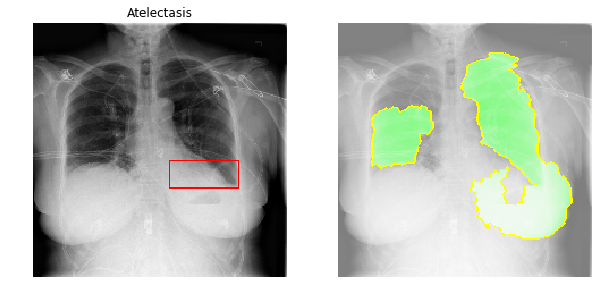
\includegraphics[width=12cm]{chapters/03_classification/images/lime_2.png}
\end{figure}

\begin{figure}[H]
\centering
\caption{Scan 8 LIME output}
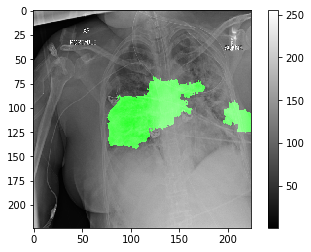
\includegraphics[width=12cm]{chapters/03_classification/images/lime_8.png}
\end{figure}

\subsection{LIME configuration}
\nblink{nhs-chest-xray/analyze/lime\_num\_features.ipynb}

\begin{figure}[H]
\centering
\caption{LIME Superpixel count: 1, 3, 6, 9}
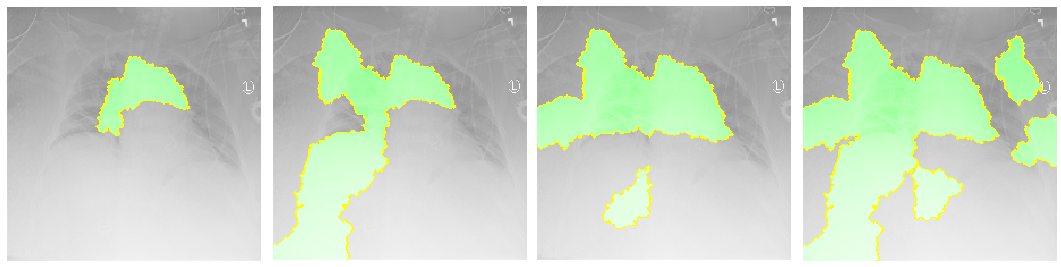
\includegraphics[width=14cm]{chapters/03_classification/images/lime-superpixel.png}
\end{figure}

\subsection{Discussion}
